\documentclass[12pt]{book}
\usepackage[utf8]{inputenc}
\usepackage[margin=1.25in]{geometry}
\usepackage{graphicx}
\usepackage{amsmath , amssymb ,ragged2e}
\usepackage{bm}
\usepackage{esvect}
\usepackage{centernot}
\usepackage[usestackEOL]{stackengine}
\usepackage{eqparbox} 
\usepackage{float}
\usepackage{siunitx}
\makeatletter
\newcommand*{\rom}[1]{\expandafter\@slowromancap\romannumeral #1@}
\makeatother

\begin{document}
    \chapter{Introduction}
        \subsection{Introduction}
            \begin{itemize}
                \item Astrologie $ \implies $ art, pas une science
                \item Astronomie $ \implies $ science d'observation et de mesures 
                \item Cosmologie $ \implies $ etude de la structure et de l'evolution de l'univers
                \item Astrophysique $ \implies $ les lois de physique vs observation
            \end{itemize}
        \subsection{Les unites de distance}
            \begin{itemize}
                \item unite astronomique (U.A.) : $ 1.\text{U.A}=1,5\times 10^{11}m $ ( pour des distances dans le systeme solaire) \\
                    1U.A = distance moyenne entre Terre soleil
                \item annee lumineuse (a.l.) : $ 1.\text{a.l.} = 63240 \text{U.A.} = 9,46\times 10 ^{15} $ ( distances entre etoiles dans la meme galaxie)
                \item parsec (pc) : $ 1.\text{pc} = 3,26.\text{a.l.}=3,1\time 10^{16} m$ ( distances entre galaxies)
            \end{itemize}
        \pagebreak
        \subsection{Systeme solaire et planetes}
            \begin{itemize}
                \item soleil
                \item mercure
                \item venus
                \item Terre
                \item mars
                \item jupiter
                \item saturne 
                \item uranus
                \item neptune
                \item pluto
            \end{itemize}
            \underline{Notes} :
            \begin{itemize}
                \item La zone habituble dans le systeme solaire et entre Venus et Mars 
                \item Tous qui est plus loin que Neptune est considere (trans neptunian objects)
                \item Notre (systeme solaire) il est a 8 Kpc du centre de la galaxie
            \end{itemize}

    \chapter{Sphere celest}
       \begin{itemize}
        \item  Sphere celeste\\
            \begin{minipage}{0.65\linewidth}
                Geocentriquement , La terre se trouve dans une spher celeste , les etoiles semblent etre fixes sur cette sphere qui tourne autour de la terre \\ 
                La terre tourne de ouest ver l'est , la sphere celest apparait en rotation d'est vers l'ouest autour de l'axe de la terre \\
                l'axe de la terre est pinte vers polaris , avec une difference de 0,75 degree
            \end{minipage}
            \begin{minipage}{0.34\linewidth}
                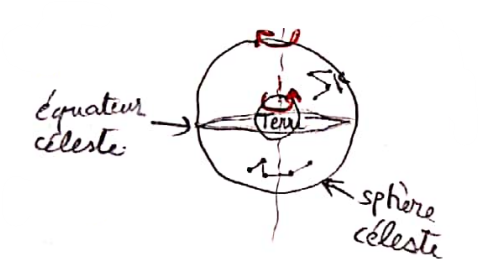
\includegraphics[width=\linewidth]{pic/spherecelest.png}
            \end{minipage}
        \item Pour determiner les coordonnees d'une etoile sur la sphere celeste , on a 2 type de coordonnees 
                \begin{itemize}
                    \item coordone locales (altitude , azimuth)\\ 
                        \begin{center}
                            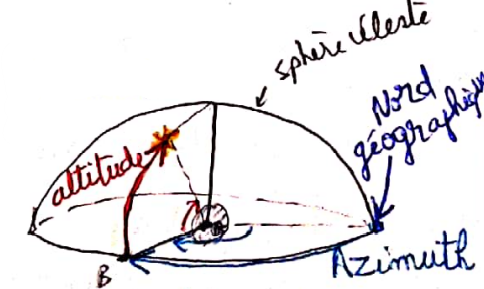
\includegraphics[width=0.3\linewidth]{pic/spherecelestcoordone1.png}
                        \end{center}
                        
                    \item coordone equatorials (dclinaison , ascension droite)\\ 
                        \begin{center}
                            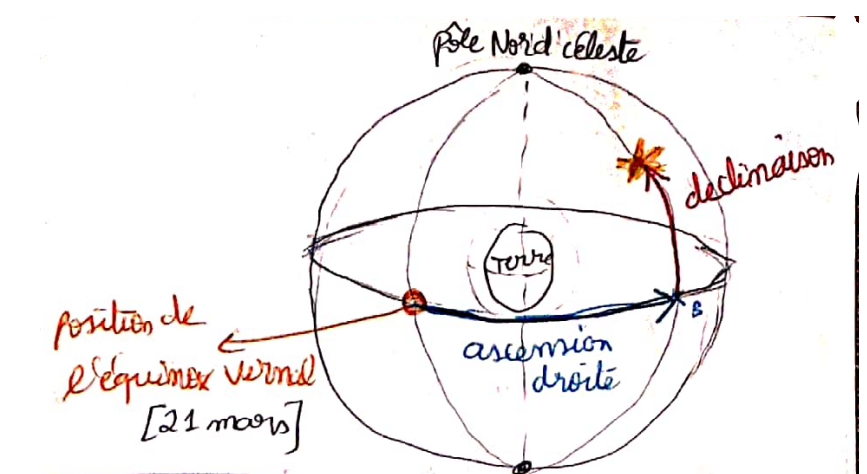
\includegraphics[width=0.3\linewidth]{pic/spherecelestcoordone2.png}
                        \end{center}
                        
                \end{itemize}
                \pagebreak
            \item Notation important
            \begin{itemize}
                \item \underline{Constellation} : groupe d'etoiles voisines , presentant une figure conventionnelle determinee , a laquelle on a donne un nom particulier 
                \item\underline{Amas (clusters)} : groupe d'etoiles liees par gravite 
                \item\underline{asterisme} : sous-groupe d'etoiles d'une constellation 
                \item\underline{etoilles (constellations) circompolaires}: ne descendent jamais sou l'horizon et peuvent etre vus toute l'annee 
                \item\underline{U.I.A.} : International Astonomical Union, designe 88 constellations dans tout le ciel
                \item\underline{eliptique} : le trajet de rotation de laterre autour du soleil \\ 
                \underline{Note :} la terre est incline par 23.5 degree $ \implies $ l'eciptique est incline par 23,5 degree par raport a l'equateur celeste 
                \item\underline{Zodiac } : ce sont 12 constellation de les 88 , les plus proches des d'ecliptique , qui sont a de largeur (18 degree ( 8 (desous de l'ecliptique)+ 8 (dessus de l'ecliptique) + 2 ( pour l'erreur)))
                \item\underline{Nominisatoin des l'etoiles selon la brillance} : $ \alpha \implies $ la plus brillante , $ \beta \implies  $ la seconde brillante ...
            \end{itemize}
       \end{itemize}
    \chapter{Les saisons}
        \begin{itemize}
            \item Mouvement de la terre 
                \begin{itemize}
                    \item Rotation (autour de son axe)
                    \item Revolution ( autour du soleil)
                \end{itemize}
            \item annee terrestre : temps mis par la terre pour effectuer 1 tour autour du soleil (365,25 jours)
            \item Jour terrestre 
                \begin{itemize}
                    \item Jour sideral : 23h 56 min : temps mis par la terre pour effectuer 1 cycle complet autour de son axe 
                    \item Jour solaire : 24 h : temps aubout duquel la terre retrouve sa position precedente par rapport a la soleil \\
                        $ J_{\text{solaire}} = J_{\text{sideral}} + 4 $
                \end{itemize}
            \item La duree du jour solaire sur une planete : $ \frac{1}{J_{\text{solair}}} = \frac{1}{J_{\text{sideral}}} - \frac{1}{A_{\text{sideral}}} $
                \begin{itemize}
                    \item  Si $ J_\text{solair} > 0 \implies  $ rotation de planete est anticlock wise
                    \item Si $ J_\text{solair} < 0 \implies  $ rotation de planete est clock wise 
                \end{itemize}
            \pagebreak
            \item L 'inclinaison de l'axe de la terre de 23,5 degree cause les saison\\
                    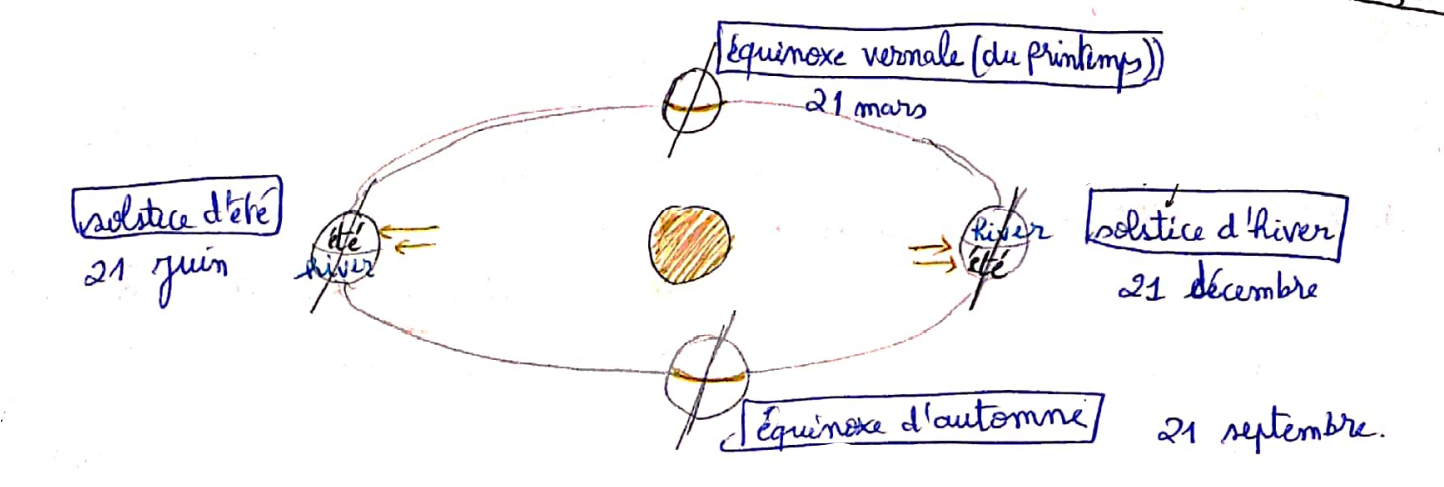
\includegraphics[width=1\linewidth]{pic/seasons.png}
                    \begin{itemize}
                        \item Pendant l'equinoxe le jour = le nuit 
                        \item Pendant le solstice d'hiver le jour < le nuit 
                        \item Pendant le solstice d'ete le jour > le nuit 
                    \end{itemize}
            \item La Terre et lune \\
                \begin{minipage}{0.65\linewidth}
                    Il existe entre la terre et la lune une forces d'attraction , maintenant , laxe de la terre pinte vers polaris ,dans 13 00 ans , il pointera vers Vega
                \end{minipage}
                \begin{minipage}{0.34\linewidth}
                    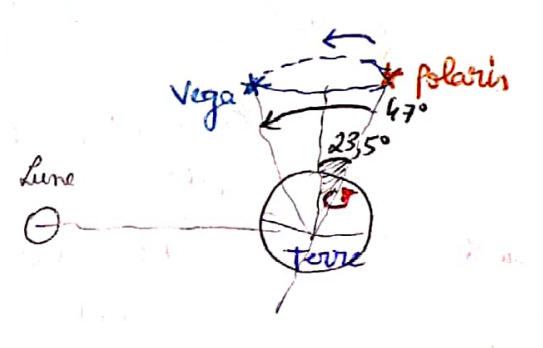
\includegraphics[width=\linewidth]{pic/vega.png}
                \end{minipage}
        \end{itemize}
    \chapter{Les eclipses}
        \begin{itemize}
            \item Eclipse lunair\\
                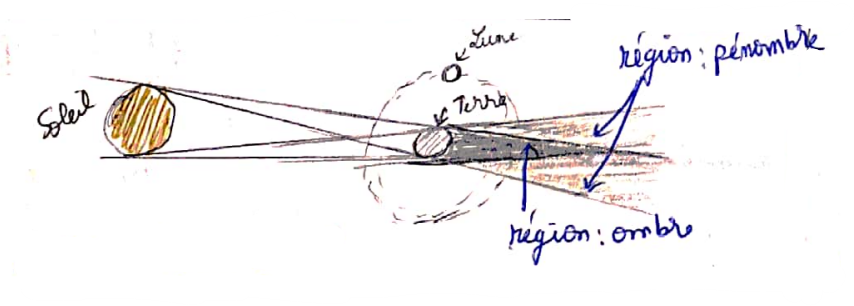
\includegraphics[width=0.7\linewidth]{pic/lunaireclipse.png}
                \begin{itemize}
                    \item penombrale : la lune est dans le penombre 
                    \item partielle : partie de la lune est dans l'ombre, l'aure partie dans le penombre 
                    \item total : la lune entiere est dans l'ombre
                \end{itemize}
                Condition de l'eclipse lunaire : \begin{itemize}
                    \item lune dans la phase "plaine lune"
                    \item Soleil , Terre et Lune alignes sur la ligne node
                \end{itemize}
            \pagebreak
            \item Eclipse solaire\\
                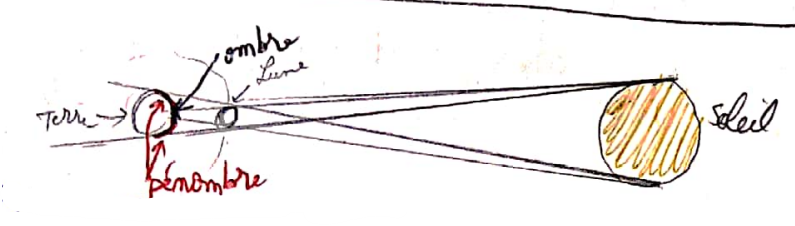
\includegraphics[width=0.7\linewidth]{pic/solaireclipse.png}
                \begin{itemize}
                    \item totale : Le sommet du cone d'ombre est sur ou au dessous de la terre 
                        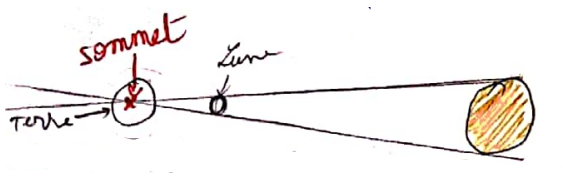
\includegraphics[width=0.3\linewidth]{pic/solareclipstotal.png}
                    \item annulaire :le sommet du cone d'ombre est au dessus de la terre \\
                        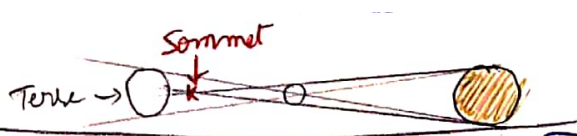
\includegraphics[width=0.3\linewidth]{pic/solareclipsannulair.png}
                \end{itemize}
                Condition de l'eclipse solaire \begin{itemize}
                    \item lune dans la phase " Nouvelle lune "
                    \item Lune Soleil , Terre alignes
                \end{itemize}
        
        \underline{Note :}Chaque 5,4 mois il y aura une eclipse (lunaire ou solaire ) a un endroit de la terre 
        \item La periodicite des eclipses : cycle saros \\
            Chaque eclipse appartient a une serie de Saros . \\
            Cycle de Saros : \\
                \begin{itemize}
                    \item la meme eclipse se pase a une periode de 18 ans + (11-$ \frac{1}{3} $)jours = 223 mois lunairs 
                    \item ces eclipse ne se produisent pas exactement au meme endroit au cours des cycle de saros 
                    \item apres 3 saros , une eclipse se produit sur la meme partie de la terre
                \end{itemize}
        \end{itemize}
    \chapter{Mouvement de la lune et ses phases}
        \begin{itemize}
            \item L'orbite de la lune est elliptique :
                \begin{center}
                    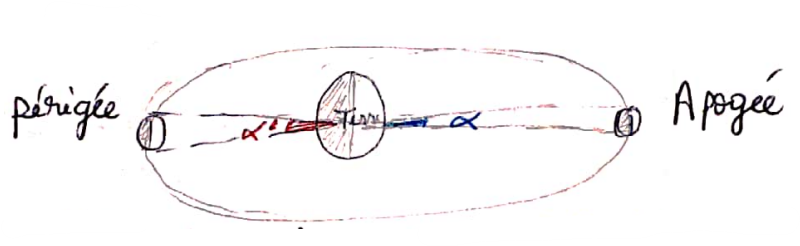
\includegraphics[width=0.5\linewidth]{pic/mouvementlune.png}
                \end{center}
            \item Quand la lune est en perigee , le diametre apparent (l'angle de vision) augmente ($ \alpha' > \alpha $ ) $ \implies $ en voit la lune plus grande 
            \item La rotation de la lune autour de son axe est lente (27 jour) 
            \item Puisque la periode de revolution de lune et la periode de rotation sont apeupres egaux $ \implies $ on voi une face unique de la lune 
            \item mois lunaire :
                \begin{itemize}
                    \item mois siderale : pour faire un cycle complete autour de la terre (27,3 jour)
                    \item mois synodique : l'intervalle entre deux nouvelles lunes (29.5 jour)
                \end{itemize} 
            \pagebreak
            \item les phases de la lune
                \begin{center}
                    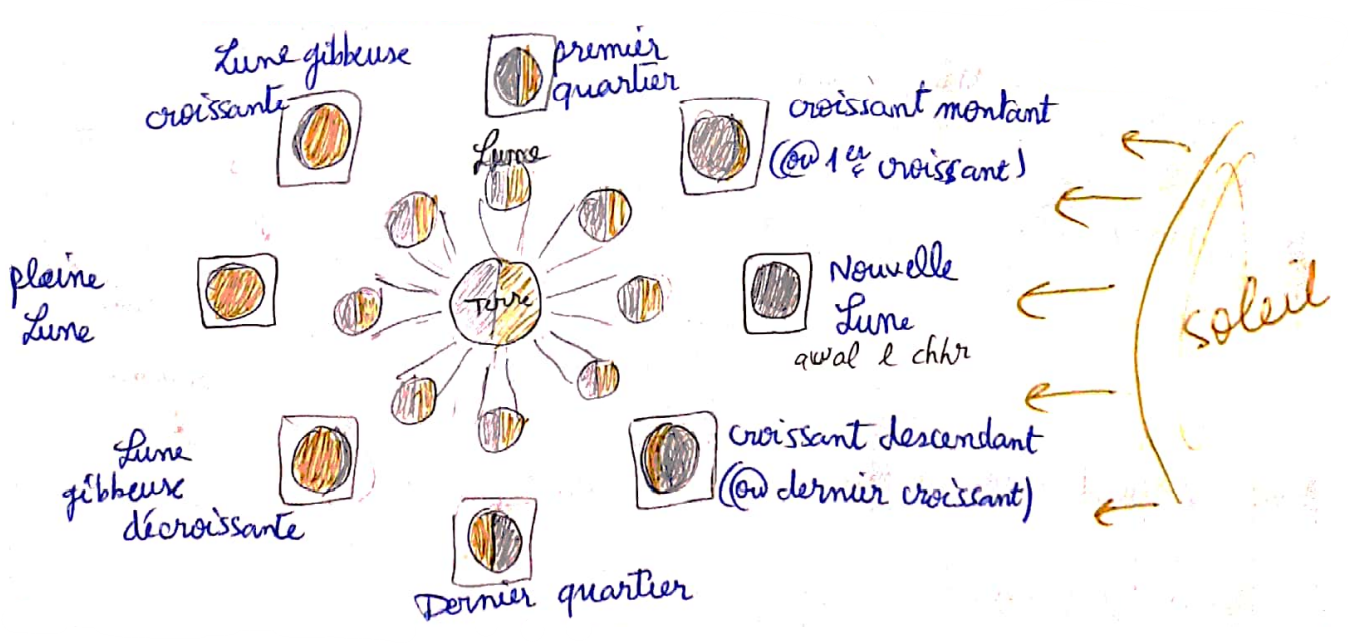
\includegraphics[width=0.8\linewidth]{pic/lunephase.png}
                        \begin{tabular}{|l|l|l|l|l|}
                        \hline
                         Phase &  Lever de la lune & coucher de la lune    \\ \hline
                         Nouvelle lune& aube  &   coucher du soleil \\ \hline
                         1er quartier& midi &    minuit\\ \hline
                         plaine lune& coucher du soleil & aube    \\ \hline
                         dernier quartier&  minuit& midi    \\ \hline
                        \end{tabular}
                \end{center}
        \end{itemize}
    \chapter{Lois des Kepler}
       \begin{itemize}
        \item  On a 3 lois de kepler :
            \begin{itemize}
                \item Les trajectoirs planetes sont elliptiques \\
                    \begin{minipage}{0.69\linewidth}
                        F1 , F2 sont des foyer \\
                        $ e = \frac{c}{a} $ est eccentricite d'une ellipse \\
                        $ 2a = AH + PH \begin{cases}
                            AH =a(1+e)\\
                            PH =a(1-e)
                        \end{cases} $
                    \end{minipage}
                    \begin{minipage}{0.22\linewidth}
                        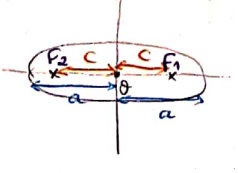
\includegraphics[width=\linewidth]{pic/kepler1.png}
                        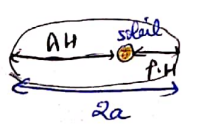
\includegraphics[width=\linewidth]{pic/kepler2.png}
                    \end{minipage}
                \item 
                    \begin{minipage}{0.79\linewidth}
                        Aires egaux pendant des temps egaux $ \implies $ La vitesse de la terre est plus grand en perihelie et plus petit en Aphelie
                    \end{minipage}
                    \begin{minipage}{0.2\linewidth}
                        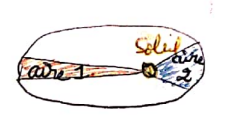
\includegraphics[width=\linewidth]{pic/kepler3.png}
                    \end{minipage}
                \item \boxed{\frac{r^3}{T^2} = \frac{G.M.}{4\pi^2}} avec $ r = a $ en general , $T$ est la periode sideral\\
                    Si $ M =$ mass solair alors \begin{itemize}
                        \item on etude une planet autour du Soleil
                        \item r en U.A.
                        \item T en annes
                        \item dans ce cas on aura $ \frac{G.M}{4\pi^2}= 1 \implies \frac{r^3}{T^2} = 1 $
                    \end{itemize}
            \end{itemize}
        \item vitess de satellisation ou vitess orbitable\\
            Pour une planet du mass (m) qui trouve autour une autre de mass (M) ona : $ v_\text{sat} = v_\text{orb} =\sqrt{\frac{G.M}{r}} $ avec r est la distance a partir du centre de (M) a (m)
        \item Vitesse du liberation \\
            pour que la planet du mass (m) qui tourne autour de (M) libert de sa orbit : $ v_\text{lib} = \sqrt{\frac{2G.M}{r}} = \sqrt{2}v_\text{sat} $
       \end{itemize}
    \chapter{Instruments Astronomiques}
       \begin{itemize}
        \item  Tout instrument astronomique a ces 2 elements essentiels 
        \begin{itemize}
            \item primaire =l objective  = collecteur (peut etre une miroir ou lentille) \\
                role : collecte la lumiere du ciel \\
                plus que le diametre de collecteur est grand on collect plus de lumier $ \implies $ plus efficacite
            \item  oculair (eyepiece) c' une lentille qui groissit les objets  
        \end{itemize}
        \item Les jumelles (Binoculars) \\
            Caracterstiques \begin{itemize}
                \item grossissement G (ou $ \delta $)
                \item objectif de diametre : D < 15cm
                \item Notation : $ G\times D $
            \end{itemize}
        \item Telescope
            On a 2 types selon le type du l'objectif 
            \begin{itemize}
                \item Telscope refracteur (tube optique , lunette astonomique)\\
                    l'objectif est une lentille \\
                    Grandissement : $ G = \frac{F}{f} $ avec $ \begin{cases}
                        F : \text{distance focale du primaire} \\ f : distance focale de l'oculaire
                    \end{cases} $
                \item Telescope Reflecteur (Telscope) \\
                    l'objectif est une miroir et on a un miroir secondaire aussi \\
                    on a 3 types de ce telescope selon la nature du miroir secondair 
                    \begin{itemize}
                        \item Newton : miroir secondaire plan 
                        \item Cassegrin : miroir secondair convexe
                        \item Gregory : miroir secondaire concave 
                    \end{itemize}
                    Grandissement : $ G = \frac{F}{f} $ avec $ \begin{cases}
                        F : \text{distance focale du primaire} \\ f : distance focale de l'oculaire
                    \end{cases} $
            \end{itemize}
            \item La magnitude visuelle maxiamle (m) qu'un telescope de diametre (D) peut detecter est : $ m = 2,7 + 5\log(D)_\text{mm} $ \\
            \item La limite de resolution ($\alpha$) : c'est la plus petit grandeur angulaire que peut distinguer un telscope (la capacite d'un système optique de mesure ) d'equation \\
                $ \alpha'' = \frac{2,5\times 10^5 .\lambda(m)}{D(m)}  $ \\
                \underline{Note:} $ \begin{cases}
                    \ang{1} = 60'(minutes)\\
                    1' = 60 '' (secondes)
                \end{cases} $\\
                Pour les telescopes optiques , dans le visible ($ \lambda \approx 555 nm $ )$ \implies \alpha'' =\frac{0,116}{D(m)} $
       \end{itemize}
    \chapter{Mesures celestes des distances}
        On a 5 methodes de Base 
        \begin{itemize}
            \item Radar (Pour les objets proches) \\
                On emet une onde electromagnetique et on mesure le temp dans laquell l'onde va et vien
                \boxed{d=c\frac{t}{2}} 
            \item Parallaxe ( methode de trangulation)  (jusqu' a 650 a.l.) \\
                C'est l'angle par lequel un objet decale quand on l'observe a partir de 2 places differentes \\
                \begin{minipage}{0.7\linewidth}
                    A est la resulta de mesur on juillet \\
                    B est la la resulta de mesur on Janvier \\
                    $ \theta : $ angle de parallaxe \\
                    $ \tan(\theta) = \frac{ST}{D} $ a chercher D
                \end{minipage}
                \begin{minipage}{0.29\linewidth}
                    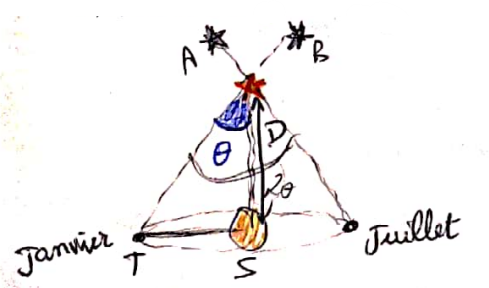
\includegraphics[width=\linewidth]{pic/parallaxe.png}
                \end{minipage}
            \item Lois de kepler ( objets orbitant une etoile)\\
                pour 2 planetes qui tournent autour du soleil : \boxed{(\frac{a_1}{a_2})^3 = (\frac{T_1}{T_2})} ( a en U.A et T en annees)
            \item Chandelle standarde  ( D $>$ 650 a.l.)\\
                \begin{itemize}
                    \item Brillance \\
                        La Brillance de surface designe la densite de flux recue par unite d'angle solide , il exsite 2 type de brillance :
                        \begin{itemize}
                            \item La \underline{ Brillance absolue}(L) Elle depend de luminosite seulment
                            \item L' \underline{ Brillance Apparent} (I) est c'est ce que nous observons , elle depend de la luminosite (L) et de la distance (r) 
                           
                        \end{itemize}
                    \item Magnitude \\
                        la magnitude est une mesure sans unite de la luminosite d'un objet celeste dans une bande de longueurs d'onde definie\\
                        \begin{itemize}
                            \item Le  \underline{Magnitude apparente} (m) mesure l'intensite\\
                                \begin{minipage}{0.49\linewidth}
                                    Plus que (m) d'une etoile augment c-a-d sa luminosite est plus faible 
                                \end{minipage}
                                \begin{minipage}{0.5\linewidth}
                                    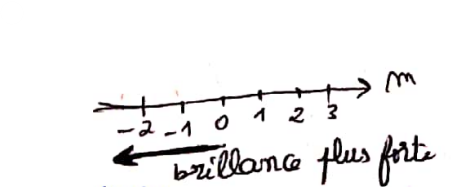
\includegraphics[width=\linewidth]{pic/magnitudeapparente.png}
                                \end{minipage}
                            \item Le  \underline{Magnitude absolue} (M) mesure la luminosite
                        \end{itemize}
                    \item Relation (Brillance - luminosite - distance) : \boxed{I=\frac{L}{4\pi r^2}}
                    \item Comparer l'intensite de 2 objets celestes : \boxed{m_1 - m_2 = 2,5\log(\frac{I_2}{I_1})}
                    \item Comparer la luminosite de 2 objets celestes : \boxed{ M_1-M_2 = 2,5\log(\frac{L_2}{L_1}) } 
                    \item La meme etoile : \boxed{m- M  =5\log(D) - 5} , D en pc 
                    \item Le rapport $ I_B/I_V$ : on compare l'intensite de lumiere recue dans le \underline{Bleu} et le \underline{Visible} jaune de meme etoile \\
                        \boxed{\frac{I_B}{I_V} = m_B-m_V \equiv B-V = 0,67 -2,5\log(\frac{I_B}{I_V})} 
                        \begin{itemize}
                            \item $ I_B/I_V > 1 \implies  $ etoile plus chaude que le soleil 
                            \item $ I_B/I_V < 1 \implies $ etoile plus froide que le soleil 
                        \end{itemize}
                        Temperature de l'etoile : \\
                            \boxed{\log(T) = 14,551 - \frac{(m_B - m_V)}{3,684}} ( la temperature T est en kelvin)
                    \item Masses des etoiles 
                        \begin{itemize}
                            \item L'etoile de plus faible masse $ \approx 0,05 M_\text{solair} $ ( 1 corps dont M $<$ 0,0$5M_\text{solair}$ n'est pas considere une etoile mais une (Brown Dwarf)) 
                            \item L'etoile de plus grande mass $ \approx 100M_\text{solair} $ (celles $>$ 100 $ M_\text{solair} $ sont incapables de maintenir leur equilibre hydrostatique $ \implies $ Supernova)  
                        \end{itemize}
                    \item Relation (Masse - Luminosite) \\
                        \boxed{\frac{L_1}{L_2} = (\frac{M_1}{M_2})^\alpha} avec $ 1<\alpha<6 $ depend de la mass de l'etoile (M) 
                    \item \underline{Note :} le magnitude du soleil : $M_\text{solair} = 4,58 ,$ Temperature de soleil : $ T_\text{solair} = 5800k , $ temp de vie de solaie : $\tau_\text{solair} = 10^{10}  $ annees
                    \item temps de vie ($ \tau $) d'une etoile de la sequence principale \\
                        \boxed{\frac{\tau}{\tau_\text{solair}} = ( \frac{M_\text{solair}}{M})^{\alpha -1 } } \\
                        ( le temp de vie est inversement proportionnel a la masse )
                    \item Radiation du corps noir : \\
                        On peut determiner la temperature d'apres la loi de WIEN  \\
                        \boxed{\lambda_{max}.T=2,9\times 10^{-3}} $m.k $ (metre . kelvin)
                    \item La loi de Stefan-Boltzmann : \boxed{I = \sigma.T^4 } , I est l'intensite emis par l'etoile par unite de surface (different que le brillance appartente)
                    \item Luminosite totale : \boxed{L = A.\sigma.T^4} , A est la surface de lobjet
                \end{itemize}
            \item Loi de hubble \\
                \boxed{D = \frac{V}{H_0} } avec $ \begin{cases}
                    V : \text{Vitesse de cette galaxie} \\ H_0 : \text{Constante de Hubble}
                \end{cases} $\\
                Pour mesurer la vitesse de la galaxie on utilise l'effet doppler ( on mesureant le shift de frequence ) par lequation : \\
                \boxed{Z =\frac{\Delta \lambda}{\lambda_0}=\frac{\lambda_r - \lambda_0}{\lambda_0} = \frac{\lambda_r}{\lambda_0} - 1 = \frac{V}{C} }$ \begin{cases}
                    Z : \text{ cosmological red shift}\\
                    V : \text{Vitesse de l'objet stellaire}\\
                    C : \text{vitesse de la lumiere dans le vide}\\
                    \lambda_r : \text{reele } \\
                    \lambda_0 : \text{observee dans le laboratoir}
                \end{cases}$\\
                \underline{Note :} cette equation valable seulement pour les cas non relativiste \\
                \begin{itemize}
                    \item si $ \lambda_r < \lambda_0 \implies V<0 \implies $ blue shift $ \implies$  la distance diminue $ \implies $ l'objet s'approche
                    \item si $ \lambda_r > \lambda_0 \implies V>0 \implies $ red shift $ \implies$  la distance augment $ \implies $ l'objet s'eloigne
                \end{itemize}
        \end{itemize}
        
    \chapter{Classification des etoiles}
        \begin{itemize}
            \item La classe spectrale (classe de temperature / couler) : \\
                \begin{center}
                    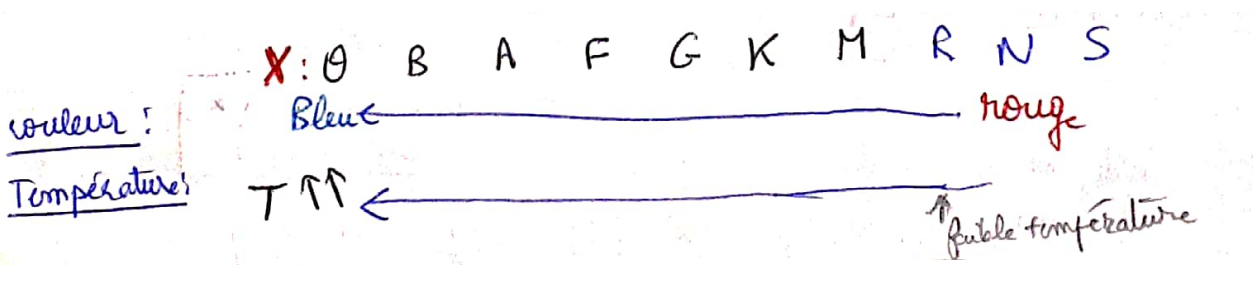
\includegraphics[width=0.8\linewidth]{pic/classspectrale.png}
                \end{center}
            \item Herzsprung Russel Diagram (HR)
                \begin{center}
                    \begin{minipage}{0.49\linewidth}
                        $ X_{ij} : \begin{cases}
                            X \implies \text{classe spectrale} \\
                            i \implies \text{ de } 0 \to 9\\
                            j \implies \text{classe de luminosite}
                        \end{cases}$ \\
                        $j \implies\begin{cases}
                            \rom{1} :\text{supergiants }\\
                            \rom{2} :\text{Bright Giants }\\
                            \rom{3} :\text{Giants }\\
                            \rom{4} :\text{Subgiants }\\
                            \rom{5} :\text{Sequence principale }\\
                        \end{cases}$
                    \end{minipage}
                    \begin{minipage}{0.5\linewidth}
                        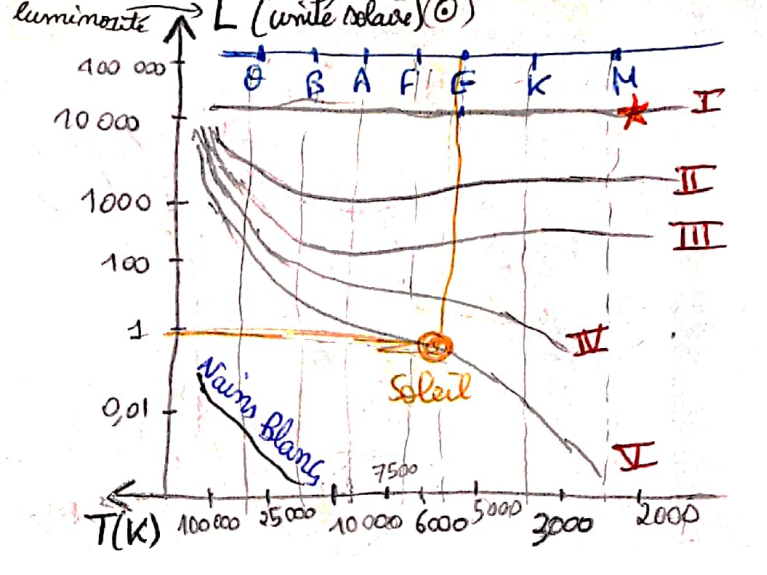
\includegraphics[width =\linewidth]{pic/herzprungdiagram.png}
                    \end{minipage}
                \end{center}
                \begin{itemize}
                    \item Masse et luminosite sont proportionnels 
                    \item La majorite des etoiles se trouvent sur la sequence principale ou elle brulent de l'hydrogene dans leurs noyaux $ \implies$ la plupart des etoiles de cette sequence sont agees [classe M]
                    \item Les mains Planes du a leurs tailles reduits , il ocupent le coin gauche en bas du diagramme HR 
                \end{itemize}
        \end{itemize}
    \chapter{Evolution des etoiles }
      \begin{itemize}
        \item   Types d'etoiles \\
        \begin{itemize}
            \item Etoiles de faible masse 
            \item Etoils de masse moyenne 
            \item Etoiles massives
        \end{itemize}
        Toutes les etoiles maissent d'une nebuleuse ( nuage de gaz) en rotation \\
        \item Protostars : \\
        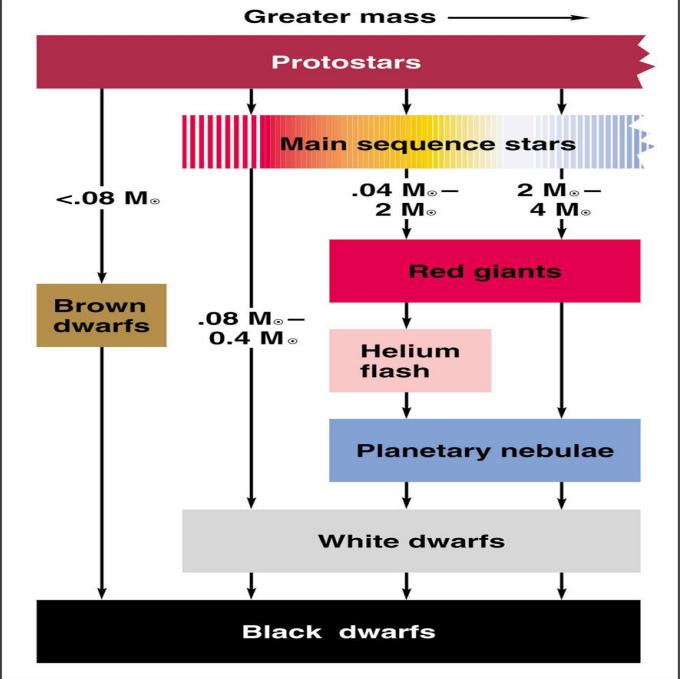
\includegraphics[width=0.7\linewidth]{pic/protostars.png} \\
        \begin{itemize}
            \item Les etoiles de masse faibles fusion le hydrogene et donne d'helium seulment 
            \item Les etoiles de masse faibles fusion le hydrogene et donne d'helium jusqua carbon et sarretent
            \item Les etoiles massive fusion le hydrogent et donne d'helium jusqua ferre
            \item Durant le supernova le bombardement des neutrons avec les noyaux forme des elements lourds (or ,uranium ...)
            \item On definit le " limite de chandraskhar " : les etoiles dont la masse du coeur restant est < 1,4 $ M_\text{solei} $ terminent leur vie pecifiquement 
            \item On definit " limite d'oppenheimer " : une limite superieure concernant la masse d'une etoile a neutrons , si elle depasse cette limite (3 $ M_\text{solei} $) elle devien un trou noir   
            \item On a ce qu'on appelle " Event Horizon " , definie par le rayon de Schubrzishild , a ce rayon , la vitesse d'echappement est c\\
                 On a $ v_\text{lib} = \sqrt{\frac{2GM}{R}}= c $ alors si on exprime la masse en masse solaires et R en Km , la formule dvient $ R=3M $\\
                 Une etoile de masse 10 masse solaire sera un trou noir si elle est comprime dans un rayon de 30 Km 
        \end{itemize}
      \end{itemize}




        
        




\end{document}